\section{Prototype data processing pipeline}

The prototype implementation of the data processing pipeline is a simplified version of the architecture described in \autoref{subsec:iot_data_pipeline}. Certain components such as \textbf{Keycloak} for authentication, geographical-based routing, and running services in a cluster have been omitted. These decisions were made to streamline development and focus on the core functionality of the system, deferring concerns like scalability and advanced security to future iterations.

The core concept remains consistent with the original design: a \textbf{queuing server} is placed behind a \textbf{reverse proxy} (using \textbf{Traefik}) to provide enhanced security and additional features such as load balancing and request routing. A \textbf{consumer} service then pulls data from the queue, performs preprocessing, and stores the processed data in a database. This approach enables modularity and ensures the data is prepared for subsequent analysis and visualization.

While the current implementation lacks certain advanced features, it retains the essential components to validate the core functionality. This includes the ability to handle incoming IoT data, preprocess it, and store it in a format optimized for the system’s use cases. The pipeline serves as a foundation for future iterations, where scalability, geographical routing, and authentication mechanisms can be incorporated.

\begin{figure}[H]
	\begin{center}
		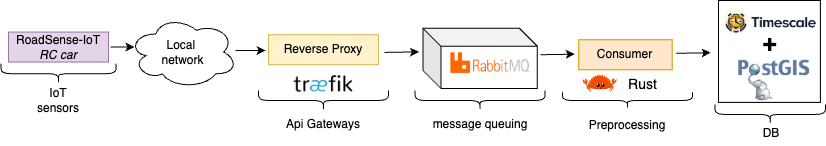
\includegraphics[width=0.95\textwidth]{../../assets/diagrams/prototype_pipeline/prototype_pipeline.png}
	\end{center}
	\caption{Prototype Data Processing Pipeline Architecture}
	\label{fig:prototype_pipeline}
\end{figure}

\noindent The communication between the IoT device and the RabbitMQ service is done using the MQTT protocol, while the consumer service uses AMQP to retrieve messages from the queue. This was done as MQTT is a lightweight protocol designed for IoT devices, making it suitable for transmitting sensor data. AMQP, on the other hand, is a robust protocol that provides additional features such as message acknowledgments and routing. The following diagram illustrated the flow of data through the prototype pipeline:

\begin{figure}[H]
	\begin{center}
		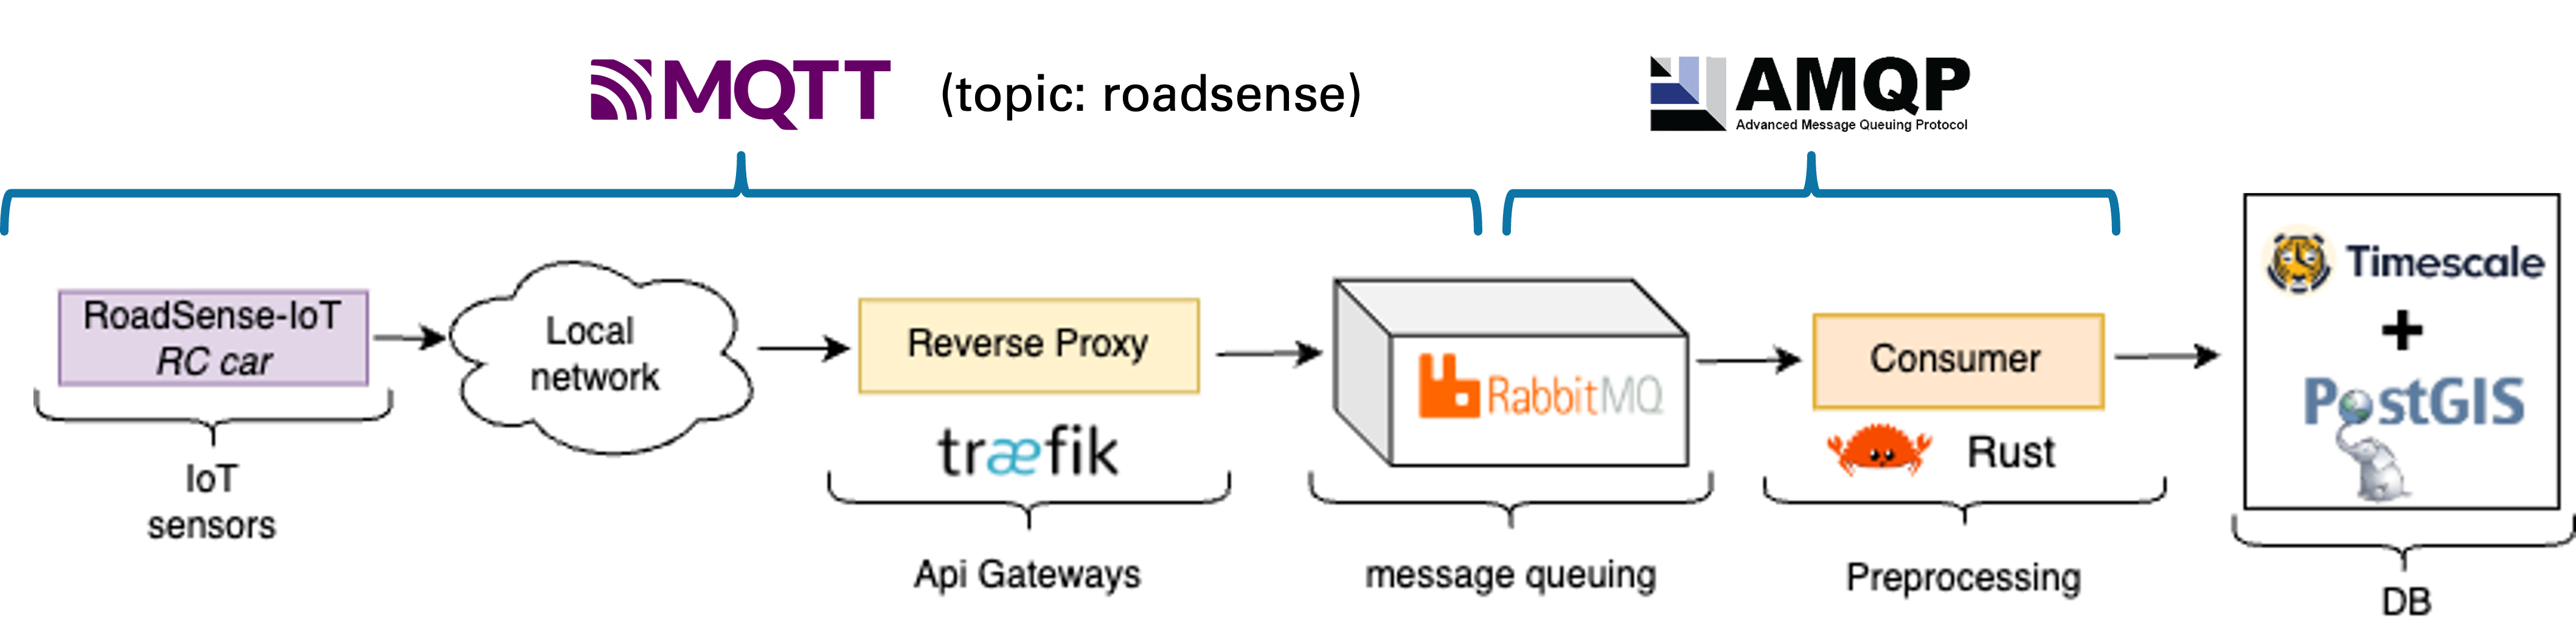
\includegraphics[width=0.95\textwidth]{../../assets/diagrams/prototype_pipeline/prototype_pipeline_annotated.png}
	\end{center}
	\caption{Prototype Data Processing Pipeline with Annotations}
	\label{fig:annotated_prototype_pipeline}
\end{figure}

\noindent This simplified implementation allows for faster prototyping and development while maintaining a clear path for future enhancements to address scalability and security concerns.
